\section{Fundamentação Teórica}
\subsection{Modelos de cores}

\begin{frame}{Introdução}
\begin{itemize}
    \item A cor tem a característica poderosa de funcionar como um descritor
    \item Os seres humanos têm a capacidade de discernir milhares de tonalidades e intensidades
    \item A percepção humana das cores se dá pela ativação de células nervosas que enviam mensagens ao cérebro sobre brilho (\textit{brightness}), matiz (\textit{hue}) e saturação (\textit{saturation})
    \item As cores podem ser especificadas por modelos matemáticos em tuplas de números em um sistema de coordenadas
    \item Dois tipos: os modelos aditivos e subtrativos
\end{itemize}
\end{frame}

%------------------------------------------------------
\begin{frame}{Modelo de Munsell}
\begin{figure}[!h]
  \centering
  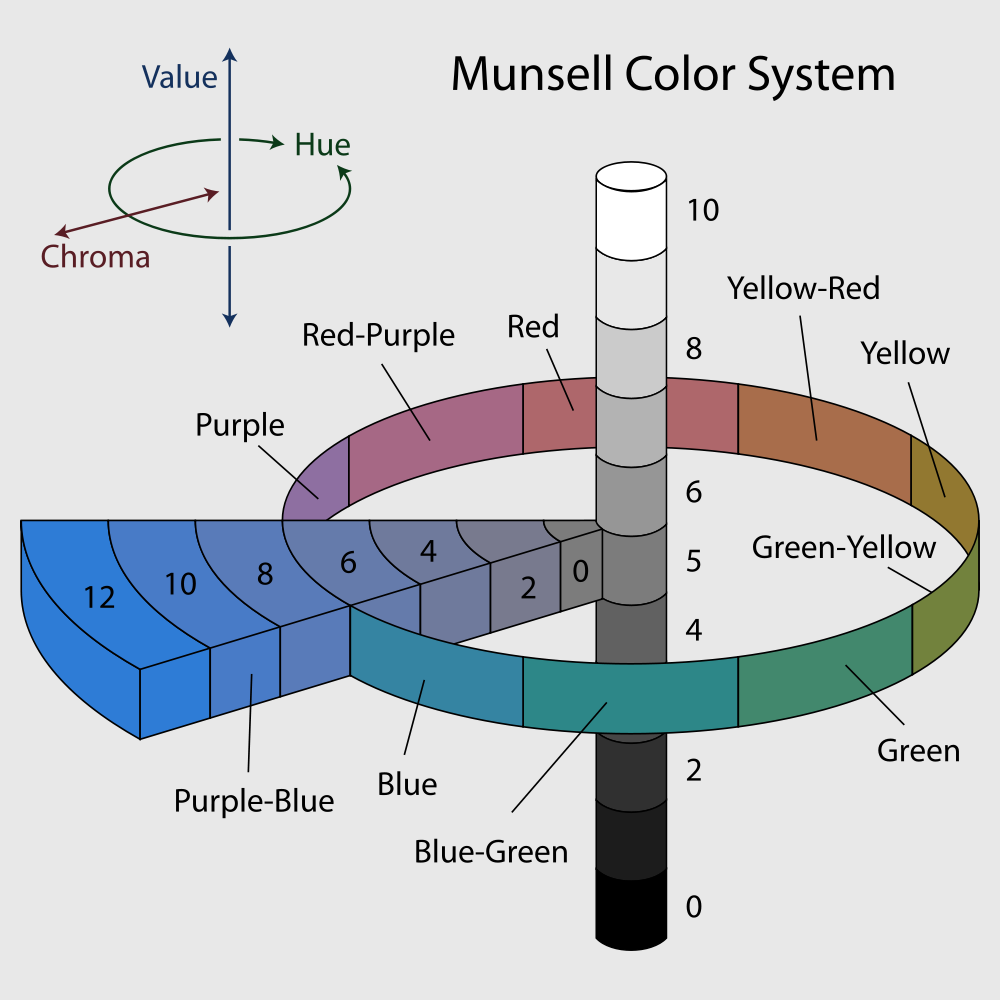
\includegraphics[width=.55\textwidth]{munsell-system}
\end{figure}
\end{frame}

%------------------------------------------------------
\begin{frame}{Diagrama de cromaticidade CIE 1931}
\begin{columns}
\column{0.5\textwidth}
\begin{itemize}
    \item Primeiro modelo matemático de especificação numérica da cor
    \item Componente de luminância Y; X e Z de cromaticidade (tristímulus)
    \item Derivações do CIE XYZ: \textbf{CIE 1976 $L^*u^*v^*$} e \textbf{1976 CIE $L^*a^*b^*$}
\end{itemize}
\column{0.5\textwidth}
\begin{figure}[!h]
  \centering
  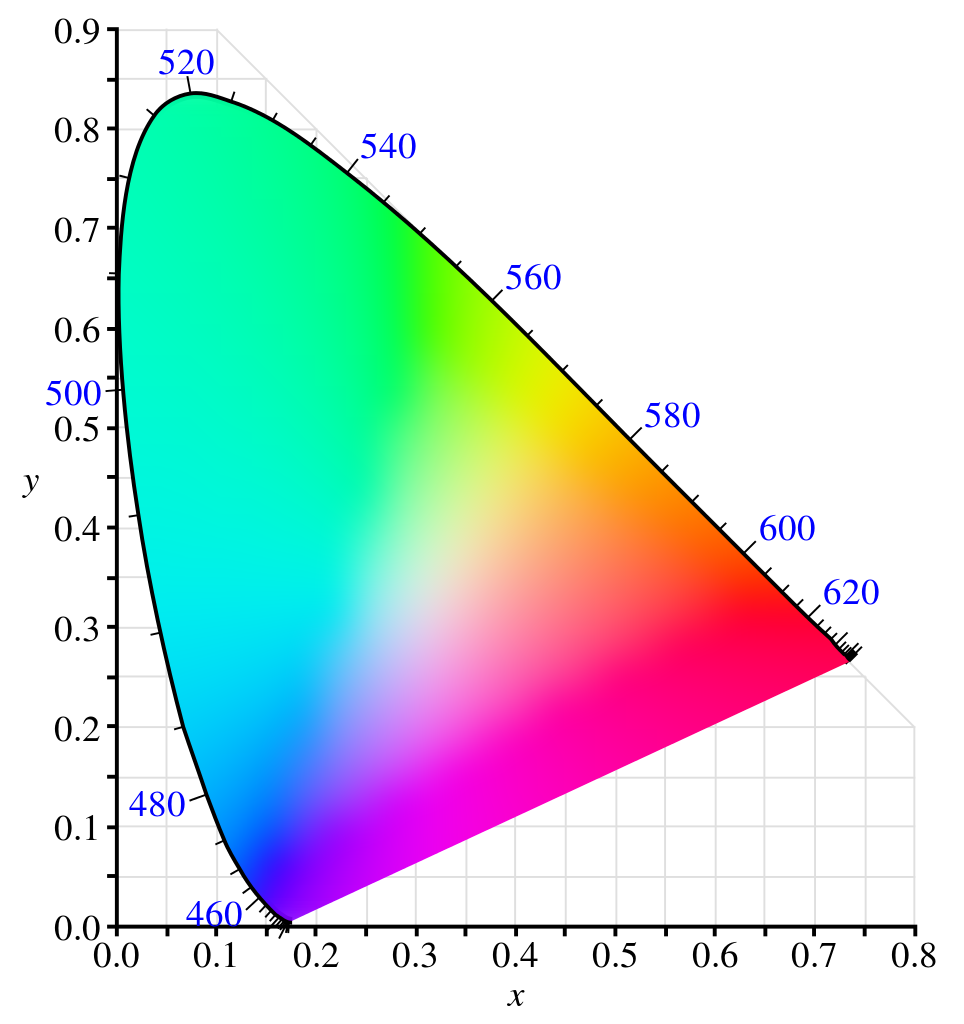
\includegraphics[width=1\textwidth]{cie-cromaticity-diagram}
\end{figure}
\end{columns}
\end{frame}

%------------------------------------------------------
\begin{frame}{Modelo RGB}
\begin{columns}
\column{0.5\textwidth}
\begin{itemize}
    \item Modelo de cores aditivo
    \item Baseado na teoria tricromática de Thomas Young e Hermann Helmholtz em meados do século 19
\end{itemize}
\column{0.5\textwidth}
\begin{figure}[!h]
  \centering
  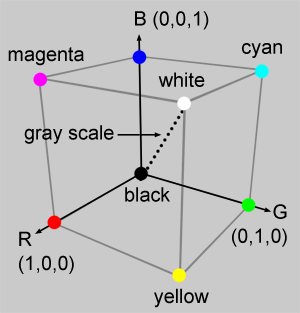
\includegraphics[width=.9\textwidth]{rgb-cube}
\end{figure}
\end{columns}
\end{frame}

%------------------------------------------------------
\begin{frame}{Modelos da família YUV}
\begin{itemize}
    \item Y = luminância, U = Azul - Y, V = Vermelho - Y
    \item Utilizado em sistemas de transmissão analógica de televisão nos padrões PAL e SECAM
    \item YCbCr é um modelo desta família e é largamente utilizado em vídeos digitais.
\end{itemize}
\begin{equation*}
  \begin{bmatrix}
    Y \\ Cb \\ Cr
  \end{bmatrix} = 
  \begin{bmatrix}
     0.299 &  0.587 &  0.114 \\
    -0.169 & -0.331 &  0.5   \\
     0.5   & -0.419 & -0.081 \\
  \end{bmatrix}
  \begin{bmatrix}
    R \\ G \\ B
  \end{bmatrix}
\end{equation*}
\end{frame}

%------------------------------------------------------
\begin{frame}{Modelos da família HSI}
\begin{itemize}
    \item  (I)ntensidade é decomposta da informação de crominância
\end{itemize}
\begin{align*}
\begin{split}
  H &=  \begin{cases}
            60\ffrac{(G - B)}{M - m}, & \text{se}\ M = R\\[0.7em]
            60\ffrac{(B - R)}{M - m} + 120, & \text{se}\ M = G\\[0.7em]
            60\ffrac{(R - G)}{M - m} + 240, & \text{se}\ M = B
       \end{cases}
  \\[0.5em]
  S &=  \begin{cases}
            \ffrac{(M - m)}{M}, \quad &\text{se}\ M \neq 0\\[0.7em]
            0, \quad &\text{caso contrário}\\
       \end{cases}
  \\[0.5em]
  V &= M
\end{split}
\end{align*}
\end{frame}

%------------------------------------------------------
\subsection{Teoria fuzzy}
\begin{frame}{Introdução}
\begin{itemize}
    \item Em muitos problemas, não há dificuldade em determinar se um dado elemento é ou não parte de um grupo
    \item $7 \in \mathbb{N}$ e $-7 \notin \mathbb{N}$
    \item Há diversos fenômenos na natureza onde a relação de pertinência não é bem definida \citep{pedrycz:98}
    \item Conjunto das pessoas altas, os números reais aproximadamente zero, o grupo de alunos mais inteligentes da escola
    \item Alto grau de incerteza inerente aos elementos e conjuntos sendo considerados
\end{itemize}
\end{frame}

%------------------------------------------------------
\begin{frame}{Introdução}
\begin{itemize}
    \item Visão tradicional e alternativa da ciência sobre a incerteza \citep{klir:95}
    \item Com base na ideia moderna de que a incerteza é algo útil na ciência, Zadeh propôs a teoria de conjuntos \emph{fuzzy}
    \item Capacidade de conjuntos \emph{fuzzy} expressarem transições graduais de pertinência e não pertinência
    \item Representação significativa e poderosa da medida de incerteza
    \item Forma de expressar conceitos vagos em linguagem natural
\end{itemize}
\end{frame}

%------------------------------------------------------
\begin{frame}{Conjuntos \emph{fuzzy}}
Da teoria de conjuntos clássicos tem-se a função característica:
\begin{equation*}
  \mu_A(x) =  \begin{cases}
                1 \quad \text{se}\ x \in A \\
                0 \quad \text{se}\ x \notin A
              \end{cases}
\end{equation*}

Que é um mapeamento dos elementos de $U$ no conjunto binário $\{0, 1\}$:
\begin{equation*}
  \mu_A =  U \rightarrow \{0, 1\}
\end{equation*}

$\forall x \in U$, se $\mu_A(x) = 1$, então $x \in A$, se $\mu_A(x) = 0$, então $x \notin A$.\\[8pt]

Em conjuntos \emph{fuzzy}, generalização aplicada no intervalo $[0, 1]$:
\begin{equation*}
  \mu_A =  U \rightarrow [0, 1]
\end{equation*}
\end{frame}

%------------------------------------------------------
\begin{frame}{Conjuntos \emph{fuzzy}}

\begin{block}{Definição de conjuntos \emph{fuzzy}}
Um conjunto \emph{fuzzy} $A$ é um subconjunto do conjunto universo $U$ formado por pares ordenados de um elemento qualquer $x$ e seu grau de pertinência dado por $\mu_A(x)$, da forma:

\begin{equation*}
  A =  \{(x, \mu_A(x)) \ |\ x \in U\}
\end{equation*}
\end{block}

As noções de inclusão, união, intersecção, complemento, relação, convexidade, etc., oriundas da teoria de conjuntos clássica, são estendidas a esses conjuntos \citep{zadeh:65}.

\end{frame}

%------------------------------------------------------
\begin{frame}{Conjuntos \emph{fuzzy}}
\begin{itemize}
    \item $U$ pode ser composto por elementos discretos ou ser um espaço contínuo
    \item A mesma implicação vale para o subconjunto $A$
    \item Quando $U$ é um conjunto discreto e finito, tal que $U = \{x_1, x_2, x_3, \ldots, x_n\}$, pode-se simplesmente enumerar os seus elementos, juntamente com seus graus de pertinência:
\begin{equation*}
  A =  \frac{\mu_A(x_1)}{x_1} + \frac{\mu_A(x_2)}{x_2} + \ldots + \frac{\mu_A(x_n)}{x_n} = \sum_{i=1}^n \frac{\mu_A(x_i)}{x_i}
\end{equation*}
\end{itemize}

\end{frame}

%------------------------------------------------------
\begin{frame}{Conjuntos \emph{fuzzy}}
\begin{block}{Definição de altura}
A altura de $A$, denotado por $altura(A)$, corresponde ao limite superior do codomínio da sua função de pertinência, da forma:
\begin{equation*}
  altura(A) = \{\mu_A(x) \ |\ x \in U\}
\label{equ:conjunto_fuzzy_altura}
\end{equation*}
\end{block}

\begin{block}{Definição de suporte}
O suporte de um conjunto \emph{fuzzy} $A$ em $U$, denotado por $suporte(A)$, é o conjunto dado por:
\begin{equation*}
  suporte(A) = \{x \in U \ |\ \mu_A(x) > 0 \}
\end{equation*}
\end{block}

\end{frame}

%------------------------------------------------------
\begin{frame}{Conjuntos \emph{fuzzy}}

\begin{block}{Definição de $\alpha$\emph{-corte} ou $\alpha$\emph{-nível}}
Um $\alpha$\emph{-corte} ou $\alpha$\emph{-nível}, é o subconjunto clássico de elementos cujo grau de pertinência é maior ou igual a um valor $\alpha$, formalmente:

\begin{equation*}
  \alpha-corte(A) = \{x \in U \ |\ \mu_A(x) \geq \alpha \}
\end{equation*}
\end{block}

\begin{block}{Definição de núcleo ou \emph{kernel}}
O núcleo ou \emph{kernel} de um conjunto \emph{fuzzy} $A$ em $U$, é o conjunto de elementos pertencentes inteiramente à $A$, da forma:

\begin{equation*}
  n\acute{u}cleo(A) = \{x \in U \ |\ \mu_A(x) = 1 \}
\end{equation*}
\end{block}

\end{frame}

%------------------------------------------------------
\begin{frame}{Representação gráfica das principais propriedades dos conjuntos \emph{fuzzy}}
\begin{figure}[!h]
  \centering
  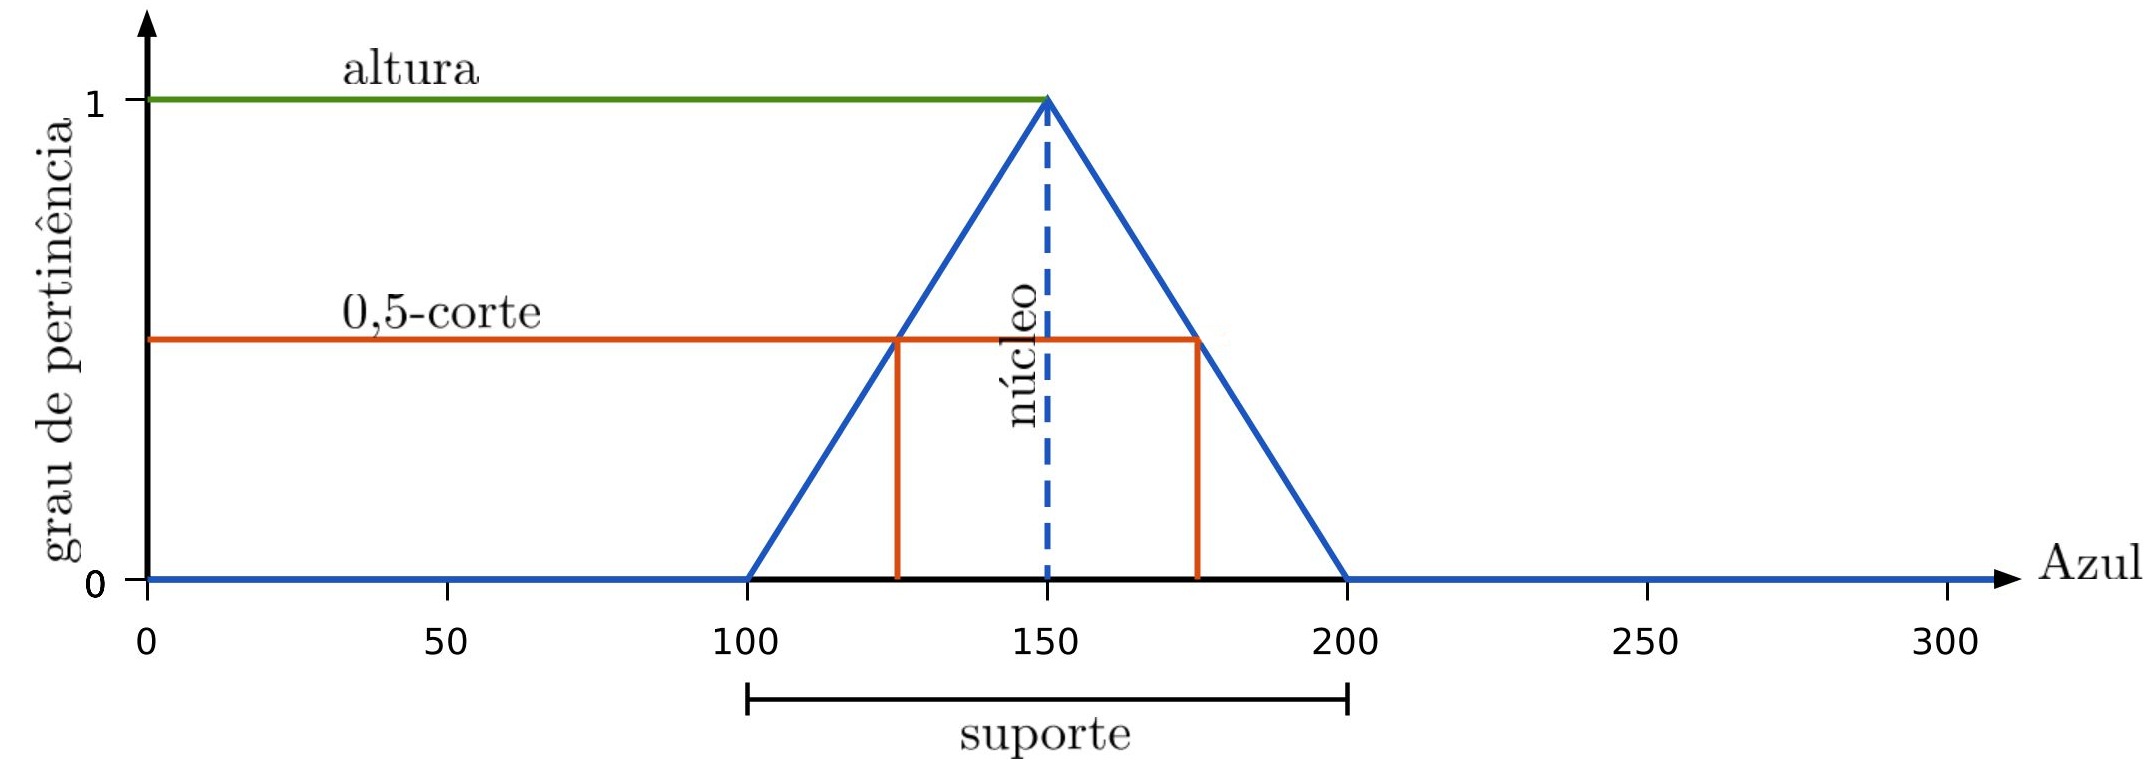
\includegraphics[width=1\textwidth]{fuzzy_definitions}
\end{figure}
\end{frame}

%------------------------------------------------------
\begin{frame}{Números \emph{fuzzy}}
Um número \emph{fuzzy} é um tipo especial de conjunto \emph{fuzzy} definido no conjunto $\mathbb{R}$ dos números reais, da forma \citep{klir:95}:
\begin{equation*}
  A : \mathbb{R} \rightarrow [0, 1]
\end{equation*}

Para que $A$ seja, de fato, um número \emph{fuzzy}, o conjunto universo no qual $\mu_A$ está definida deve ser $\mathbb{R}$ e as seguintes propriedades devem ser satisfeitas \citep{barros:06}:

\hspace{4pt}(i) todos os $\alpha$\emph{-corte} de $A$ são não vazios, com $0 \leq \alpha \leq 1$\\
\hspace{2pt}(ii) todos os $\alpha$\emph{-corte} são intervalos fechados de $\mathbb{R}$\\
(iii) $suporte(A) = \{x \in U \ |\ \mu_A(x) > 0\}$

\end{frame}

%------------------------------------------------------
\begin{frame}{Funções de pertinência}
Um número \emph{fuzzy} $A$ é dito triangular se sua função de pertinência, denotada por $\mu_{A}(x)$, é da forma:

\begin{columns}
\column{0.5\textwidth}
\begin{equation*}
  \mu_A(x) =  \begin{cases}
                \ffrac{x - a}{m - a}, &\text{se}\ a < x \leq m\\[0.5em]
                \ffrac{b - x}{b - m}, &\text{se}\ m < x < b\\[0.5em]
                0, &\text{c.c.}
              \end{cases}
\end{equation*}

\column{0.5\textwidth}
\begin{figure}[!h]
  \centering
  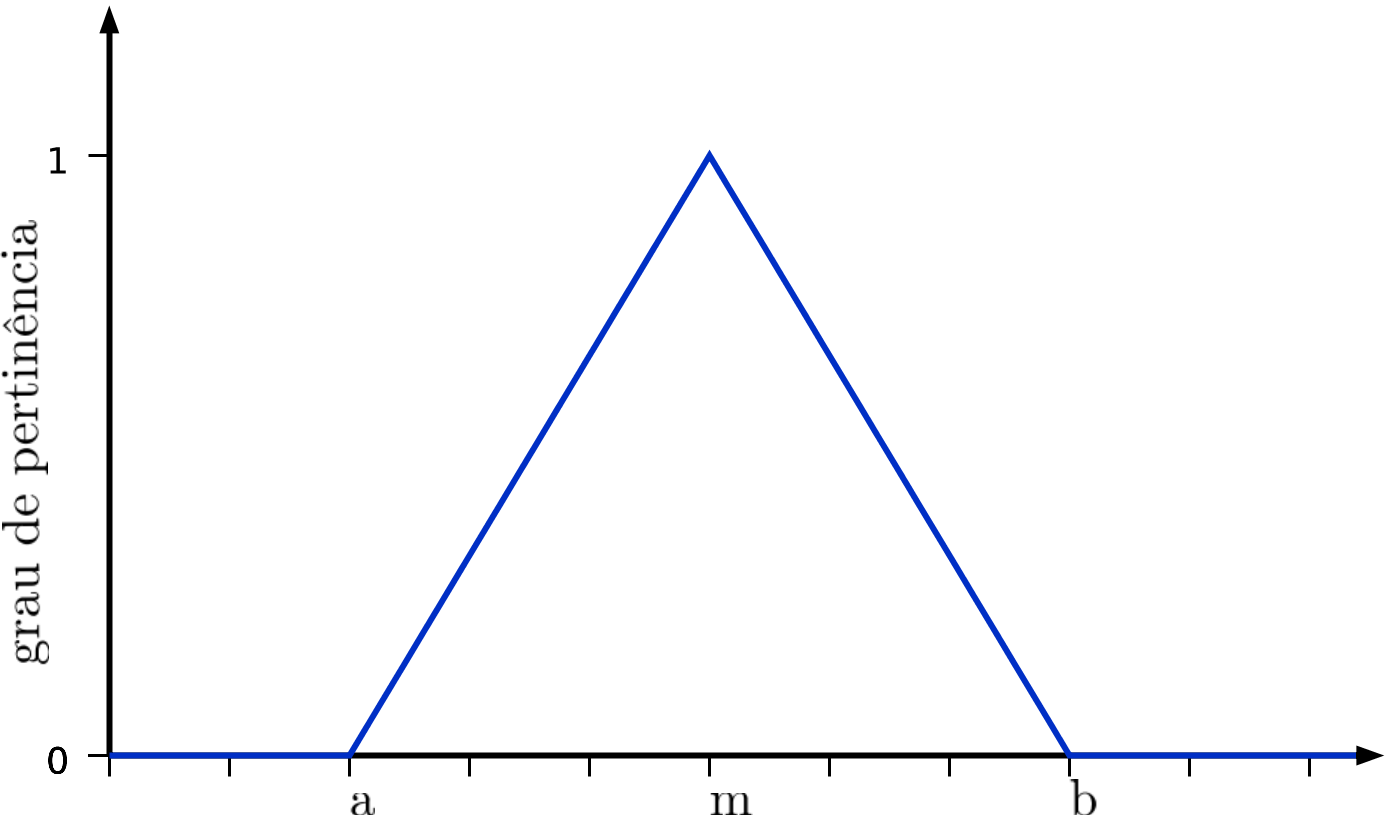
\includegraphics[width=1\textwidth]{funcao_triangular}
\end{figure}
\end{columns}
\end{frame}

%------------------------------------------------------
\begin{frame}{Funções de pertinência}
Um número \emph{fuzzy} $A$ é dito trapezoidal se sua função de pertinência, denotada por $\mu_{A}(x)$, é da forma:

\begin{columns}
\column{0.5\textwidth}
\begin{equation*}
  \mu_A(x) =  \begin{cases}
                \ffrac{x - a}{b - a}, & \text{se}\ a < x < b\\[0.5em]
                1, & \text{se}\ b \leq x \leq c\\[0.5em]
                \ffrac{d - x}{d - c}, & \text{se}\ c < x < d\\[0.5em]
                0, & \text{c.c.}
              \end{cases}
\end{equation*}

\column{0.5\textwidth}
\begin{figure}[!h]
  \centering
  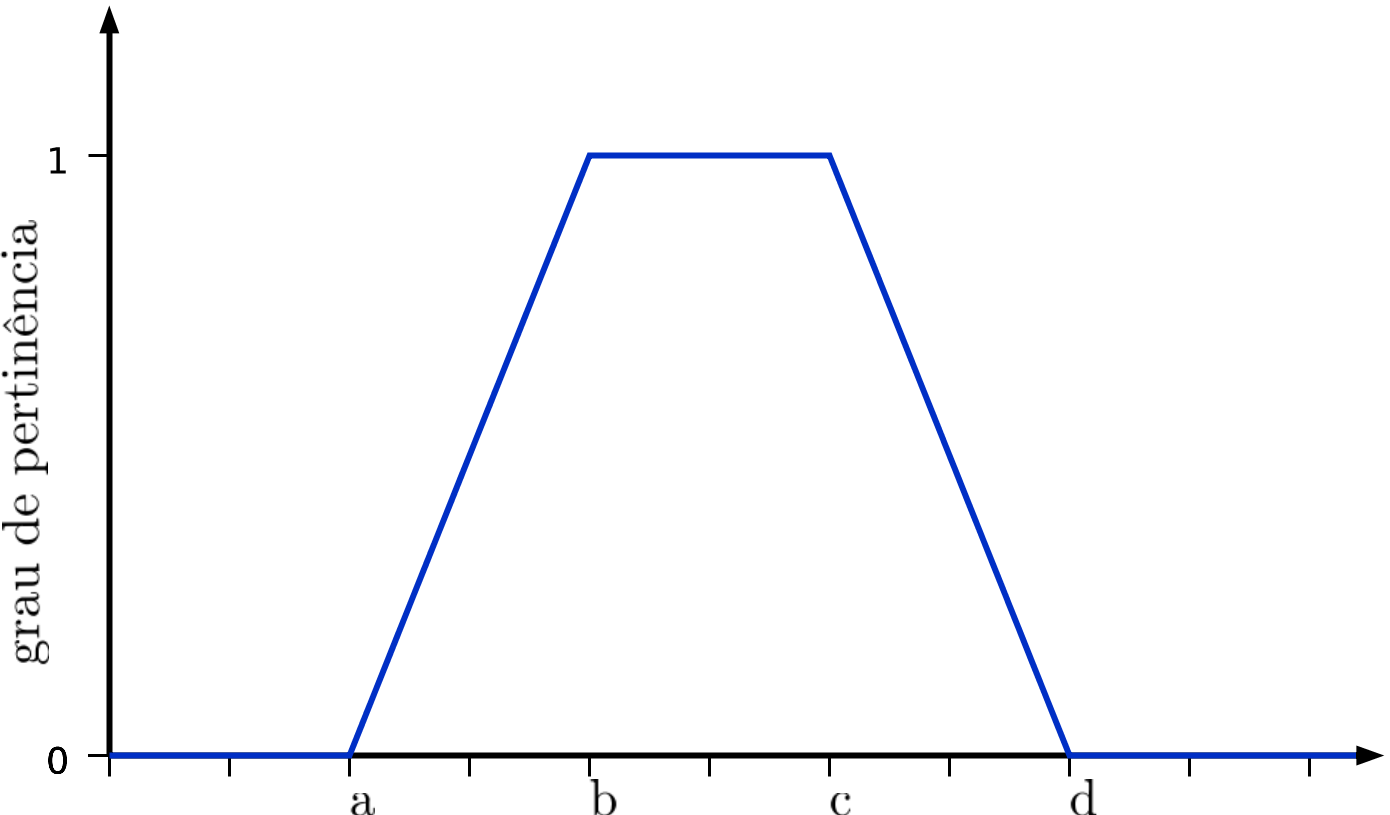
\includegraphics[width=1\textwidth]{funcao_trapezoidal}
\end{figure}
\end{columns}
\end{frame}

%------------------------------------------------------
\begin{frame}{Funções de pertinência}
Um número \emph{fuzzy} $A$ é dito gaussiano se sua função de pertinência, denotada por $\mu_{A}(x)$, é da forma:

\begin{columns}
\column{0.5\textwidth}
\begin{equation*}
  \mu_A(x) =  \begin{cases}
                \exp{\big(-\ffrac{{(x - m)}^2}{\sigma} \big)}, \\ \text{se}\ m - \sigma \leq x \leq m + \sigma\\[0.5em]
                0, \ \text{c.c.}
              \end{cases}
\end{equation*}

\column{0.5\textwidth}
\begin{figure}[!h]
  \centering
  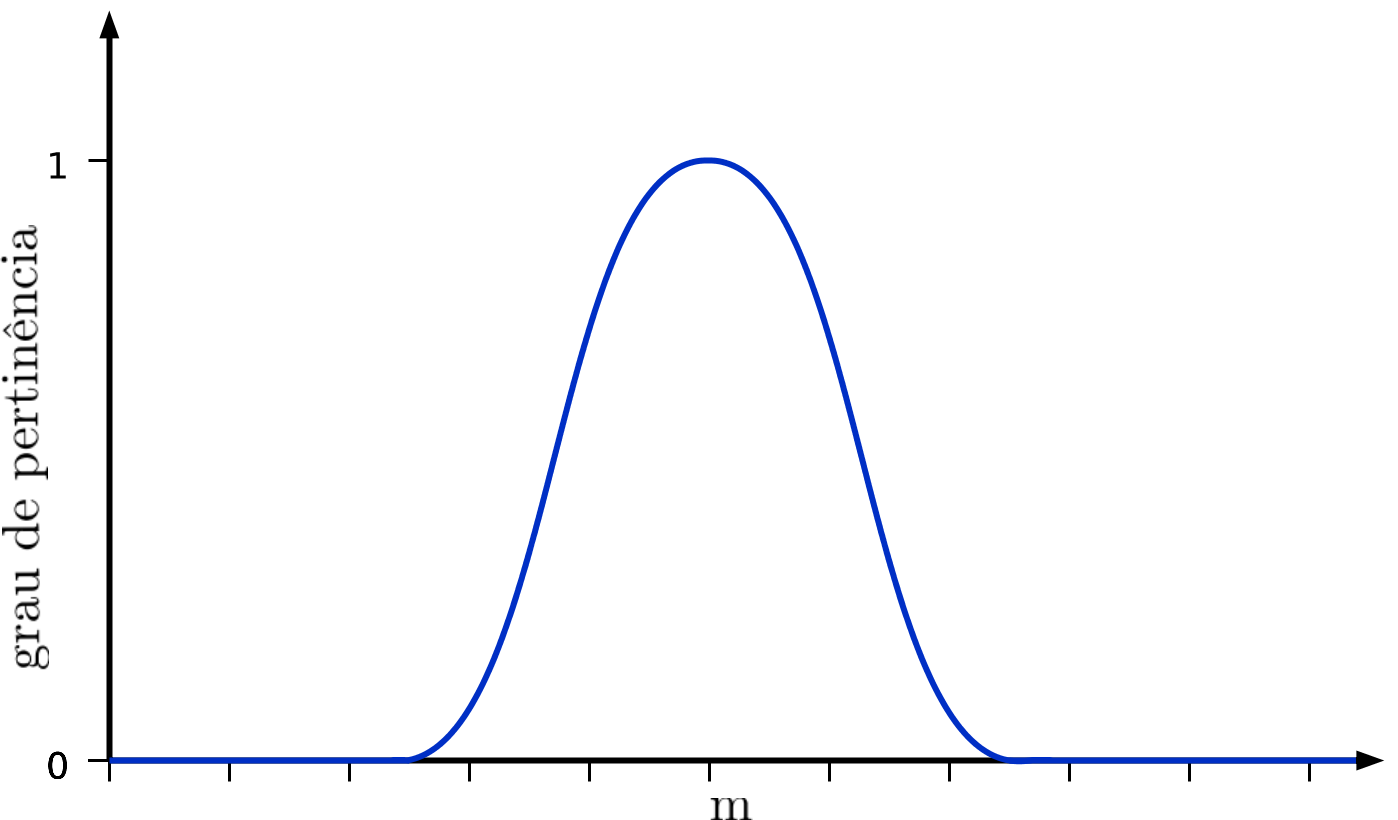
\includegraphics[width=1\textwidth]{funcao_gaussiana}
\end{figure}
\end{columns}
\end{frame}

%------------------------------------------------------
\subsection{Classificadores}
\begin{frame}{Máquinas de Vetores Suporte (SVM)}
\end{frame}

%------------------------------------------------------
\begin{frame}{$k$-Vizinhos Mais Próximos ($k$-NN)}
\end{frame}

%------------------------------------------------------
\begin{frame}{Árvores de decisão}
\end{frame}